\chapter{Conclusion}
\label{chapter:conclusion}

%\minitoc
\chapterwithfigures{\nameref*{chapter:conclusion}}
%\chapterwithtables{\nameref*{chapter:introduction}}

\ifthenelse{\boolean{skipConclusion}}{\endinput}{}

This thesis primarely focused on the novel view synthesis issue, mostly with the highly constrained single-view scenario. We skim through in this section over our core contributions, before drawing up  the current 2024 landscape in \ac{IA} and 3D. The last section of this manuscript will be devoted to the perspectives and further work this PhD thesis might lead to. 

\section{Contributions}

This manuscript has adressed in a large extend the single-image \ac{NVS} issue. We built in our first two contributions around latest deep learning architectures to synthesize a novel viewpoint of a static scene from a single source posed image. Our latest project has an industrial primary aim, where novel views are rendered from a scene that was explicitly reconstructed in 3D as a gaussian point cloud.

We started this manuscript by presenting in Chapter \ref{chapter:epipolarnvs} our epipolarNVS architecture. Our main motivation through this work was to propose an innovative way to encode camera pose information in an image-to-image \ac{CNN} for \ac{NVS}. Whereas most of prior work often discretized \citep{kim2020novel} or encoded camera pose information into a low dimensional signal \citep{sun2018multiview}, we rather exploited the epipolar constraint to encode such prior signal. Through a vanilla grid sampling strategy on the source view, we project epipolar lines on a blank RGB image, that was been fed alongside the source image to pose-condition the network. 

We then investigated in Chapter \ref{chapter:epinerf} how epipolar constraints could be bring into a generalizable \ac{NeRF} architecture for single-image \ac{NVS}. Based on \textit{source-aligned} dense feature volume produced from a CNN-encoder, we trained a novel \ac{NeRF}-architecture, termed NeRFeature \ref{subsec:epinerf/method/nerfeature} to produce \textit{target-aligned} features. These \textit{source} and \textit{target-aligned} feature are finally used through an epipolar constraint in a light attention mechanism. We extensively shown in the devoted Experiments section \ref{subsec:epinerf/experiments} how our three-stage training architecture might help generalizable \ac{NeRF}s to better perfrom on single-image \ac{NVS} task.  

Finally, Chapter \ref{chapter:gausssplat} has been entirely devoted to the \ac{NVS} solution we started investigated with CarCutter by Meero few months ago. The camera spin stabilization algorithm allows to render from a 3D \ac{GS} reconstructed scene novel viewpoints which were initially uncomplete and cropped (subsection \ref{subsec:gs-vanilla_gs}). We presented a bunch of improvements to go beyond this first reconstruction in Experiments \ref{sec:gs-experiment}. However, 3D \ac{GS}-based scenes remain prone to floaters artifact when they are rendered at non-training locations. We will push in that direction in a close future to develop a floater removal algorithm. While results are still unperfect for an industrial application, research and open-source projects around \ac{GS} \citep{kerbl20233d} are tremendously prolific and move at a very steady pace for 10 months now \citep{luiten2023dynamic,yang2024gaussianobject,wewer24latentsplat}. 

On top of these contributions, we also introduce in Appendix \ref{chapter:appendix} our very first work, called AdaptativeSR \citep{landreau2022adaptativesr}. There is no direct relationship with the \ac{NVS} but rather with topological considerations in low-resolution 3D meshe structure. Idea was to leverage on the very first differentiable rasterizers that emerged in 2020 \cite{liu2019soft} (before this PhD started) to prune faces of a genus-0 object mesh. By solely relying on 2D binary rendered silhouette mask of such a 3D object, we proposed an effective yet imperfect algorithm to adapt mesh topology. 

\section{IA challenges in 2024}

This section embrasses the most recent issues and trends 3D related \ac{IA} landscape is currently living. This section is not technical but aims to span across the main challenges the scientific community - from academic researchers to tech companies -, but also individuals, will have to face in the months and years to come. 

\subsection{Open-source}
We can reliably claim that \ac{IA} has been bring into world hands with the release by OpenIA in December 2022 of ChatGPT, an \ac{LLM} based conversational chabot. 

Pour autant, la technologie derrière les LLM n'était pas intégralement nouvelle, et OpenIA avait pour habitude de publier régulièrement des notes techniques de ces recherches, ainsi que le code source associé en accès libre. OpenIA était ainsi extrèmement permissive quant à l'usage de GPT-2 \citep{radford2019language}, version antérieure de 2018 à ChatGPT. Une telle époque est désormais révolu chez OpenAI, qui ne publie en open source que très peu de ses produits (à l'image de Whisper, general-purpose speech recognition model). Avec une rapidité déconcertante, un véritable chisme à eu lieu dans l'industrie de l'IA, mettant dos à dos les entreprises vantant et défendant ardement l'open source et celle étant convaincu de la nécessité de garder sa technology pour soit. Des entreprises, qui sont pour là plus part davantage de très jeunes startup,  telles que Mistral IA, HuggingFace ou StableDiffusion,  s'opposent désormais à des entreprises qui vendent et distribuent un produit dont la technologie est entièrement fermée au monde académique, à l'image de d'OpenIA, ou d'Antropic ou de MidJourney. 

A titre personnel, je pense intimmement que la recherche en IA est désormais supporté par une communauté si brillante techniquement et si motivée intellectuellement par les challenges à venir, que les entreprises faisant le choix déliberé de développer uniquement en interne leur produit IA se feront, à très court terme, rattrapé et dépassé. La Figure \ref{fig:conclusion-openclose} illustre d'ailleurs en un sens ce propos, à minima pour le domaine des LLMs. 
 
\begin{figure}[htb!]
    \center
  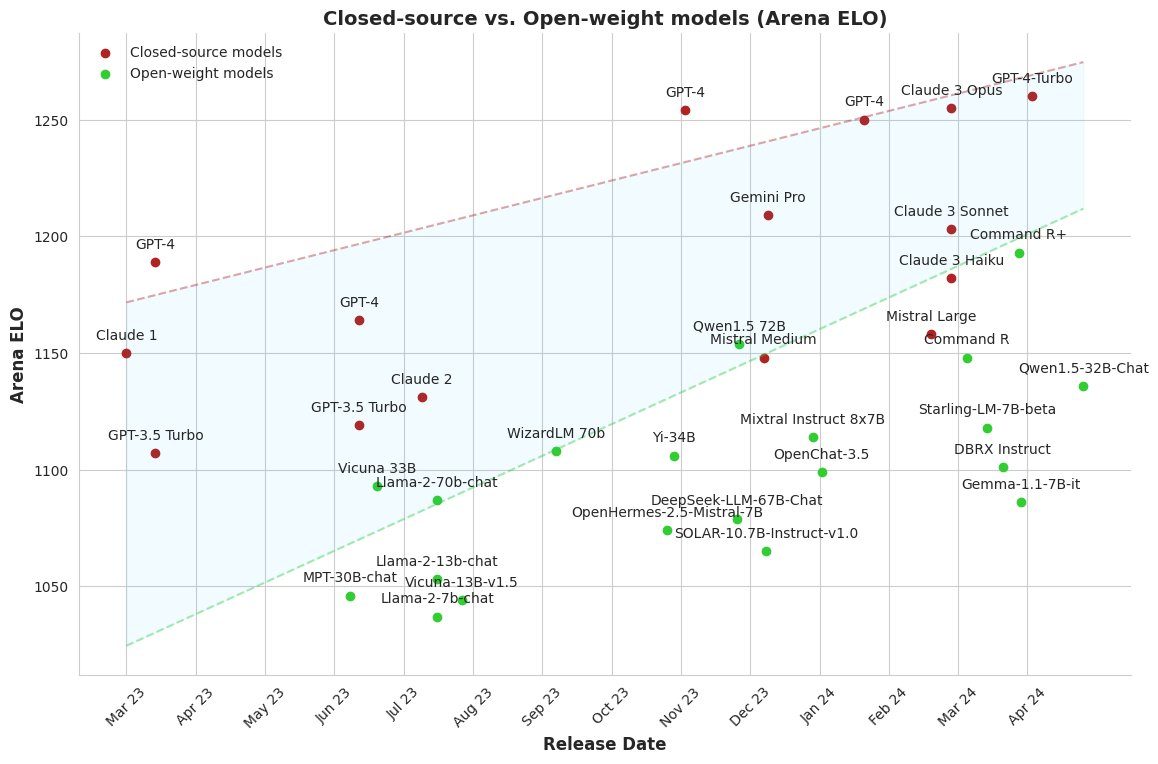
\includegraphics[width=\linewidth]{images/conclusion/open-close.jpeg}
  \caption{\textbf{LLMs ELO score based on human ratings.} Such graphs is built on a regular monthly basis thanks to \citep{chiang2024chatbot} work. It seems that open models now has a 6 to 10-month lag, againt more than years when GPT-4 was released.}
  \label{fig:conclusion-openclose}
\end{figure}

Bien que moins marqué que les LLMs par cette tendance, le monde de la 3D voit lui aussi son lot d'entrepises défendant l'un de ces deux modèles. StabilityIA, déjà plus que largement connu et reputé dans le monde de l'image en IA grâce à ces modèles de diffusion \citep{esser2024scaling}, a ainsi très récement rendu public un nombre important de modèles de reconstruction 3D \cite{TripoSR2024 ,voleti2024sv3d} à partir d'une image. 


\subsection{Fundation models and environmental issue}
Cependant, bien que qu'un nombre croissant de modèles soit librement accessible, les ressources GPUs requises pour pouvoir entrainer et ou utiliser ces modèles, aux dizaines voir centaines milliards de paramètres, demeurent très souvent énormes, voire gargantuesques. 


Factorial Funds estime ainsi qu'il a fallu, pour entrainer le dernier modèle de texte to vidéo d'OpenIA, nommé SoRA, entre 4.2k et 10K H100 GPUs sur un mois entier. A raison d'une consomation de 700W par GPUs, l'entrainement de SoRA aura donc consommé autant d'électrcité qu'un francais moyen en 12 ans. Toujours selon le même rapport, extrement documenté et accessible ici, il est estimé qu'un seul H100 sera capable de générer 5 minutes de vidéo par heure. Si une telle technologies vise dans l'année à venir à être accessible publiquement, Factorial Funds estime qu'il faudra près de 720k H100 à OpenIA pour répondre à une demande mondiale, en assumant que 50\% des vidéos postés sur TikTok et 15\% des vidéos sur Youtube seront gérés via un tel modèle.

Et la tendance n'est pas, de la part d'NVIDIA qui a le monopole sur la production des GPUs, à un développement de GPUs frugale d'un point de vue de la consomation électrique. L'actuelle finallité est davantage tournée vers le nombres d'opérations que de telles machines peuvent faire à la seconde: la consomation électrique de la prochaine génération d'architecture Blackwell d'NVIDIA, avec les B100s semble être donnée à 1000W. 

Toutes les modalités, du texte,à l'audio, en passant par l'image, la vidéo et donc la 3D auront leur modèle de fondation. La 3D est peut être désormais le seul domaine qui n'a pas encore son modèle de fondation à l'heure où ces lignes sont écrites, mais il ne s'agit là que d'une question de temps. Sam Altman affirme d'ailleurs sur X, en Avril 2024, "movies are going to become video games and video games are going to become something unimaginably better". 

\subsection{Ethics & Harmness}

\section{Perspectives and further work}
\subsection{Trends and application in 3D}
\subsection{Further work}

